\documentclass{report}
\usepackage{amsmath,amssymb,amsthm,textcomp,gensymb,nccmath}
\usepackage{mathtools}
\renewcommand{\qedsymbol}{$\blacksquare$}

\setlength{\topmargin}{0.5in}
\usepackage[margin=4cm]{geometry}
\usepackage{enumerate}

\usepackage{setspace}
\onehalfspacing
\usepackage{parskip}
\setlength{\parskip}{0.5em}
\usepackage[T1]{fontenc}
\usepackage{palatino}

% useful characters/operators
\newcommand{\R}{\mathbb{R}}
\newcommand{\C}{\mathbb{C}}
\newcommand{\Z}{\mathbb{Z}}
\newcommand{\Q}{\mathbb{Q}}
\newcommand{\N}{\mathbb{N}}
\newcommand{\F}{\mathbb{F}}
\newcommand{\B}{\mathbb{B}}
\newcommand{\matP}{\mathbb{P}}
\newcommand{\matE}{\mathbb{E}}
\newcommand{\matS}{\mathbb{S}}
\newcommand{\matH}{\mathbb{H}}
\newcommand{\matT}{\mathbb{T}}
\newcommand{\st}{\ s.t.\ }
\newcommand{\ie}{\ i.e.\ }
\newcommand{\eg}{\ e.g.\ }
\def \diam {\operatorname{diam}}
\def \Hom {\operatorname{Hom}}
\def \id {\operatorname{id}}
\def \tr {\operatorname{tr}}
\def \rk {\operatorname{rk}}
\def \sp {\operatorname{span}}
\def \dist {\operatorname{dist}}
\def \intr {\operatorname{int}}
\def \sgn {\operatorname{sgn}}
\def \im {\operatorname{Im}}
\def \re {\operatorname{Re}}
\def \curl {\operatorname{curl}}
\def \divg {\operatorname{div}}
\def \GL {\operatorname{GL}}
\def \Aut {\operatorname{Aut}}
\def \per {\operatorname{per}}
\def \LE {\operatorname{LE}}
\def \indeg {\operatorname{indeg}}
\def \outdeg {\operatorname{outdeg}}
\def \Par {\operatorname{Par}}
\def \Gr {\operatorname{Gr}}
\def \del {\operatorname{del}}
\def \add {\operatorname{add}}
\def \Gal {\operatorname{Gal}}
\def \Sym {\operatorname{Sym}}
\def \dist {\operatorname{dist}}
\newcommand{\pdr}[2]{\dfrac{\partial #1}{\partial #2}}
\newcommand{\df}{\mathrm{d}}
\newcommand{\idf}{\ \mathrm{d}}
\newcommand{\dr}[2]{\dfrac{\df #1}{\df #2}}
\newcommand{\inner}[2]{\left\langle #1, #2\right\rangle}
\newcommand{\qbin}[2]{\begin{bmatrix}{#1}\\ {#2}\end{bmatrix}_q}
\newcommand{\into}{\hookrightarrow}
\newcommand{\onto}{\twoheadrightarrow}
\newcommand{\from}{\leftarrow}
\newcommand{\norm}[1]{\left\| #1 \right\|}
\newcommand{\floor}[1]{\left\lfloor #1 \right\rfloor}
\newcommand{\set}[1]{\left\{ #1 \right\}}
\newcommand{\rank}{\operatorname{rank}}

% arrows and :=, =:
\makeatletter
\providecommand*{\twoheadrightarrowfill@}{%
  \arrowfill@\relbar\relbar\twoheadrightarrow
}
\providecommand*{\twoheadleftarrowfill@}{%
  \arrowfill@\twoheadleftarrow\relbar\relbar
}
\providecommand*{\xtwoheadrightarrow}[2][]{%
  \ext@arrow 0579\twoheadrightarrowfill@{#1}{#2}%
}
\providecommand*{\xtwoheadleftarrow}[2][]{%
  \ext@arrow 5097\twoheadleftarrowfill@{#1}{#2}%
}
\makeatother

\newcommand{\defeq}{\vcentcolon=}
\newcommand{\eqdef}{=\mathrel{\mathop:}}

% integral for measure theory
\newcommand{\lowerint}{\underline{\int_{\R^d}}}
\newcommand{\upperint}{\overline{\int_{\R^d}}}
\newcommand{\lint}[1]{\underline{\int_{\R^d}} #1 (x)dx}
\newcommand{\uint}[1]{\overline{\int_{\R^d}} #1 (x)dx}
\newcommand{\sint}[1]{\simp{\int_{\R^d} #1 (x)dx}}
\newcommand{\lesint}[1]{\int_{\R^d} #1 (x)dx}

% note taking
\newcommand{\fancyem}[1]{\underline{\textsc{#1}}}

% theorem style
\newtheorem{theorem}{Theorem}[section]
\newtheorem{corollary}{Corollary}[section]
\newtheorem{lemma}{Lemma}[section]
\newtheorem{conjecture}{Conjecture}[section]
\newtheorem{proposition}{Proposition}[section]

\theoremstyle{definition}
\newtheorem{definition}{Definition}[section]
\newtheorem{example}{Example}[section]
\theoremstyle{remark}
\newtheorem*{remark}{Remark}

% pseudocode and algorithms
\usepackage{algorithm}
\usepackage{algpseudocode}
\usepackage{algorithmicx}
\counterwithin{algorithm}{section}
\renewcommand{\algorithmicrequire}{\textbf{Input:}}
\renewcommand{\algorithmicensure}{\textbf{Output:}}

% for clearer reference
\usepackage{hyperref}
\newcommand{\corollaryautorefname}{Corollary}
\newcommand{\lemmaautorefname}{Lemma}
\newcommand{\definitionautorefname}{Definition}
\newcommand{\exampleautorefname}{Example}
\newcommand{\conjectureautorefname}{Conjecture}
\renewcommand{\subsectionautorefname}{Section}
\newcommand{\algorithmautorefname}{Algorithm}

% other styling
\usepackage{fancyvrb, fancyhdr}
\usepackage{tikz-cd}
\usepackage{tikz}
\PassOptionsToPackage{usenames, x11names}{xcolor}
\usepackage{tcolorbox}
\selectcolormodel{cmy}

\newcommand{\edge}{
    \begin{tikzcd}[cramped, sep=small, labels={font=\everymath\expandafter{\the\everymath\textstyle}}]
        u \arrow[r, "e", no head] & v
    \end{tikzcd}
}


\pagestyle{fancy}
\fancyhead[LO,L]{\leftmark}
\fancyhead[RO,R]{Yiwei Fu}
\fancyfoot[CO,C]{\thepage}
\renewcommand{\sectionmark}[1]{\markboth{#1}{#1}}

\numberwithin{equation}{section}

\newcommand{\fnl}{\parbox[t]{0\linewidth}{}}
\newcommand*\ttlmath[2]{\texorpdfstring{$\boldsymbol{#1}$}{#2}}

\usepackage{epigraph}

% \epigraphsize{\small}% Default
\setlength\epigraphwidth{8cm}
\setlength\epigraphrule{0pt}

\usepackage{etoolbox}

\makeatletter
\patchcmd{\epigraph}{\@epitext{#1}}{\itshape\@epitext{#1}}{}{}
\makeatother

% combinatorics special
\usepackage{pgfopts}
\usepackage{ytableau}



\begin{document}
\title{Notes for Math 669}
\author{Yiwei Fu, Instructor: Alexander Barvinok}
\date{FA 2022}
\maketitle


\tableofcontents
Office hours: 

\clearpage
\pagenumbering{arabic}


\chapter{Introduction to Lattices}
\section{Definition}
\begin{definition}
    A lattice $\Lambda \subset V$ is a discrete additive group.
\end{definition}

\section{Lattice and Its Basis}
Last time: $L \in V$ is a subspace if $L = \operatorname{span} (L \cap \Lambda)$

\begin{theorem}
    If $L$ is a lattice subspace, $L \neq V$, then $\exists u \in L \setminus \Lambda$ such that $d(u, L) \leq d(x, L)$ for all $x \in L \setminus \Lambda$.
\end{theorem}

Say $L \in \operatorname{span}\left\{u_1, \ldots, u_m\right\}$ linearly independent vectors, $\Pi = \left\{\right\}$ There is $u \in \Lambda \setminus L$ such that $\dist(u, \Pi) \leq \dist(x, \Pi)$ for all $x \in \Lambda \setminus L$. 
\begin{proof}
    Take $\rho > 0$ large enough. Consider $\Pi_\rho = \left\{y, d(y, \Pi) \leq \rho\right\}$. It contains points from $\Lambda \setminus L$, choose the one in $\Pi_\rho \cap (\Lambda \setminus L)$ closet to $\Pi$.
\end{proof}
\fancyem{Claim} $u \in \Lambda \setminus L$ is what we need. Why?
Pick any $x \in \Lambda \setminus L$. Let $y \in L$ be the closest to $x$. 
\[\dist(x, L) = \norm{x - y} = \norm{(x - w) - (y - w)}.\]
\[y = \sum_{i=1}^m d_iu_i\]
Let $w = \sum_{i=1}^m \floor{\alpha_i}u_i \in \Lambda \setminus L, y - w = \sum_{i=1}^m \set{\alpha_i}u_i \in \Pi$. 

\begin{theorem}
    Every lattice has a basis.
\end{theorem}
\begin{proof}
    By induction on $n = \dim V$.
    
    \textbf{Base case:} for $n = 1$, we have $V = \R$.

    Let $u > 0$ be the lattice vector closet to $0$, among all positive vectors in $\Lambda$.

    Then $u$ is a basis of $\Lambda$. Pick any $v \in \Lambda$. Assume $v > 0$ WLOG. Then $v = \alpha u$ for $\alpha > 0$. If $\alpha \in \Z$ then we are done. If not, consider $w = \alpha u - \floor{\alpha} u = \set{\alpha} u$, this is closer to $0$ than $u$, a contradiction.

    \textbf{Induction hypothesis:} suppose any lattice of dimension $n - 1$ has a basis.

    \textbf{Induction step:} pick a lattice hyperplane $H$ (lattice subspace with $\dim = n - 1$). Then $\Lambda_1 = H \cap \Lambda$ has a basis $u_1, \ldots, u_{n-1}$. Pick $u_n$ such that $u_n \notin H$ and $\dist(u_n, H)$ is the smallest. We claim that $u_1, \ldots, u_{n-1}, u_n$ is a basis of $\Lambda$.

    Let $u \in \Lambda$, $u = \sum_{i=1}^n \alpha_i u_i$ with $\alpha_i \in \R$. If $\alpha_n = 0$ then $u \in \Lambda_1$, then $\alpha_1, \ldots, \alpha_{n-1} \in \Z$. Suppose $\alpha_n \neq 0$. Consider $w = u - \floor{\alpha_n}u_n$. $w \in \Lambda$ and $w = \set{\alpha_n}u_n + \sum_{i=1}^{n-1} \alpha_i u_i$. So \[\dist(w, H) = \dist(\set{\alpha_n}u_n, H) = \set{\alpha_n}\dist(u_n, H)\] If $\set{\alpha_n} > 0$ then $0 < \dist(w, H) < \dist(u_n, H)$, a contradiction.

    So $\set{\alpha_n} = 0 \implies \alpha_n \in \Z$. Then $w = \sum_{i=1}^{n-1} \alpha_i u_i \implies \alpha_1, \ldots, \alpha_{n-1} \in \Z$.

    So we have constructed a basis for lattice of dimension $n$, thus finishing the proof.
\end{proof}


This is called A.N.Korkin(e)-Zolotarev(öff) basis.

\fancyem{Exercise} Suppose $u_1, \ldots, u_n \in V$ is a basis of subspace. The integer combinations form a lattice.

\fancyem{Exercise} Suppose a $2$-dimensional lattice. Then there exists a lattice basis $u, v$ such that the angle $\alpha$ between $u, v$ satisfies $\frac{\pi}{3} \leq \alpha \leq \frac{\pi}{2}$.

\fancyem{Exercise} If $\Lambda$ is a lattice and $L$ is a lattice subspace. The orthogonal projection $\operatorname{PR}: V \to L^{\perp}$. Then $\operatorname{PR}(\Lambda) \subset L^\perp$ is a lattice.

\begin{definition}
    Suppose $u_1, \ldots, u_n$ be a basis of $\Lambda$. 
    \[\Pi=\set{\sum_{i=1}^n \alpha_i u_i: 0 \leq \alpha_i < 1, i = 1, \ldots, n}\] is the \emph{fundamental parallelepiped} of a fundamental parallelepiped of $\Lambda$.
\end{definition}
\begin{theorem}
    The volume of a fundamental parallelepiped $\Pi$ doesn't depend on $\Pi$. The volume is called the determinant of $\Lambda$. Furthermore, if $B_{r} = \set{x: \norm{x} \leq r}$, then \[\lim_{r \to \infty} = \frac{|B_r \cap \Lambda|}{\operatorname{vol}B_r} = \frac{1}{\det \Lambda}.\]
\end{theorem}
We start with a lemma:
\begin{lemma}\label{le:1.1.1}
    Let $\Pi$ be a fundamental parallelepiped of $\Lambda \subset V$. Then every vector $x \in V$ is uniquely written as $x = u + y$ where $u \in \Lambda, y \in \Pi$.
\end{lemma}
\begin{proof}
    Existence: $\Pi$ is the fundamental parallelepiped for $u_1, \ldots, u_n$. If $x = \sum_{i=1}^n \alpha_i u_i$ then $u = \sum_{i=1}^n \floor{\alpha_i} u_i$ and $y = \sum_{i=1}^n \set{\alpha_i} u_i$

    Uniqueness: suppose $x = u_1 + y_1 = u_2 + y_2$ then $u_1 - u_2 = y_2 - y_1$. Since $u_1 - u_2 \in \Lambda$ we have $y_2 - y_1 = \sum_{i=1}^n (\alpha_i - \beta_i)\mathbf{u}_i$. We have $(\alpha_i - \beta_i) \in \Z$. Since $-1 < \alpha_i - \beta_i < 1$, it has to be $0$.
\end{proof}
A geometry interpretation is that we can cover the whole space with fundamental parallelepipeds without overlaps.

\newcommand{\vol}{\operatorname{vol}}

\begin{proof}[Proof of theorem]
    Let \[X_{r} = \bigcup_{u \in B_r \cap \Lambda} (\Pi + u)\]
    Then $\operatorname{vol} X_r = |B_r \cap \Lambda| \operatorname{vol}\Pi$.

    Say, $\Pi \subset B_a$ for some $a > 0$. Then $X_r \subset B_{r + a}$.
    Look at $B_{r - a}$. It is covered by $\Pi + u: u \in \Lambda$. We should have $\norm{u} \leq r$. Hence $B_{r - a} \subset X_r$.

    So we have \[\left(\frac{r-a}{a}\right)^n = \frac{\vol B_{r-a}}{\vol B_r} \leq \frac{\vol X_r}{\vol B_r} \leq \frac{\vol B_{r+a}}{B_r} = \left(\frac{r+a}{a}\right)^n\]

    This goes to 1 when $r \to \infty$.
\end{proof}

\fancyem{Remark/Exercise} The same holds for balls not centered in the origin: \[B_{r}(x_0) = \set{x: \norm{x - x_0} \leq r}.\]

\fancyem{Exercise} Suppose a lattice $\Lambda \subset V$ and $u \in \Lambda$. The Voronoi (G.F. Voronoi, 1868-1908) region is defined by \[
\Phi_{u} = \set{x \in V: \norm{x - u} \leq \norm{x-v}, \forall v \in \Lambda}.  
\]
Show that $\Phi$ is convex (bounded by at most $2^n$ affine hyperplanes) and $\vol \Phi = \det \Lambda$.

\fancyem{Exercise} $(\det \Lambda)(\det \Lambda^*) = 1$

\section{Sublattice}
\begin{definition}
    Suppose $\Lambda \subset V$ is a lattice, and $\Lambda_0 \subset \Lambda, \Lambda_0 \subset V$ is also a lattice. $\Lambda_0$ is then called a sublattice of $\Lambda$.
\end{definition}
\begin{remark}
    We have $\rank \Lambda_0 = \rank \Lambda$.
\end{remark}
\begin{example}
    $D_n \subset \Z^n$.
\end{example}
$\Lambda$ is an Abelian group and $\Lambda_0 \subset \Lambda$ is a subgroup. Look at the quotient $\Lambda/\Lambda_0$ and cosets $\set{u + \Lambda_0}$. The index of $\Lambda_0$ in $\Lambda |\Lambda / \Lambda_0| = $ the number of cosets.

\begin{theorem}
    \begin{enumerate}
        \item Let $\Pi$ be a fundamental parallelepiped of $\Lambda_0$ Then $|\Lambda / \Lambda_0| = |\Pi \cap \Lambda|$.
        \item $|\Lambda /\Lambda_0| = \dfrac{\det \Lambda_0}{\det \Lambda}$.
    \end{enumerate}
\end{theorem}
\begin{proof}
    \begin{enumerate}
        \item By \autoref{le:1.1.1}, every coset has a unique representation in $\Pi$.
        \item Let $B_r = \set{x: \norm{x} \leq r}$. Then \[\lim_{r \to \infty} = \frac{|B_r \cap \Lambda|}{\vol B_r} = \frac{1}{\det \Lambda}.\]
        Let $S \subset \Lambda$ be the set of coset representatives. Then $|S| = |\Lambda/\Lambda_0|.$ Then $\Lambda = \bigcup_{u \in S} (u + \Lambda_0)$. Hence \[\lim_{r \to \infty} \frac{|B_r \cap (u + \Lambda_0)|}{\vol B_r} = \frac{1}{\det \Lambda_0}. \implies \frac{1}{\det \Lambda} = |S|\frac{1}{\Lambda_0}\qedhere\]
    \end{enumerate}
\end{proof}

\fancyem{Exercise} \begin{enumerate}
    \item $\det \Z^n = 1$
    \item $\det D_n = 2$.
    \item $\det D^+_n = 1$. ($n$ even)
    \item $\det A_n = \sqrt{n+1}$. $\det E_8 = 1, \det E_7 = \sqrt{2}, \det E_6 = \sqrt{3}$.
    \item If $a_1, \ldots, a_n$ are coprime integers not all $0$. \[\Lambda = \set{(x_1, \ldots, x_n) \in \Z^n: a_1x_1 + \ldots + a_nx_n = 0} \text{ has } \det \Lambda = \sqrt{a_1^2 + \ldots + a_n^2}.\] 
\end{enumerate}

\begin{corollary}
    If $u_1, \ldots, u_n \in \Lambda$ are linearly independent and \[\vol \set{\sum_{i+1}^n \alpha_iu_i: 0 \leq \alpha_i < 1} = \det \Lambda\] then $u-1, \ldots, u_n$ is a basis.
\end{corollary}
\begin{proof}
    Look at \[\Lambda_0 = \set{\sum_{i=1}^n m_iu_i: m_i \in \Z}, |\Lambda/\Lambda_0| = 1 \implies \Lambda = \Lambda_0 \qedhere\]
\end{proof}

Counting integer points. Suppose $\Lambda = \Z^n$.

Pick $n$ linearly independent vectors $u_1, \ldots, u_n \in \Lambda$. Consider \[\Pi = \set{\sum_{i=1}^n \alpha_iu_i: 0 \leq \alpha_i < 1}.\] Then \[
    |\Pi \cap \Z^n| =\ ?    
\]
Suppose $\Lambda_0 = \set{\sum_{i=1}^n m_iu_i: m_i \in \Z}$. Then $\det \Lambda_0 = \vol \Pi$.

Suppose $n = 2$, $u_1 = (3, 1), u_2 = (1, 2)$. Then $\vol \Pi = 5$. We can see that the  parallelogram contains 5 integer points.

\[
\begin{tikzpicture}
    \draw[thick, -stealth](-1,0) -> (xyz cs:x=5);
    \draw[thick, -stealth](0,-1) -> (xyz cs:y=4);
    \draw[step=1cm,gray,very thin] (0,0) grid (4, 3);
    \draw[red, thick] (0, 0) -- (1, 2);
    \draw[red, thick] (0, 0) -- (3, 1);
    \draw[red, thick, dashed] (1, 2) -- (4, 3);
    \draw[red, thick, dashed] (3, 1) -- (4, 3);
    \node[shape=circle, fill=black, scale = 0.5] () at (0, 0) {};
    \node[shape=circle, fill=black, scale = 0.5] () at (1, 1) {};
    \node[shape=circle, fill=black, scale = 0.5] () at (2, 1) {};
    \node[shape=circle, fill=black, scale = 0.5] () at (2, 2) {};
    \node[shape=circle, fill=black, scale = 0.5] () at (3, 2) {};
\end{tikzpicture}    
\]

The case for $n = 2$ is special. 
\begin{theorem}[Pick Formula (G.A. Pick, 1859-1942)]
    If $P \subset \R^2$ is a convex polygon with integer vertices and non-empty interior. Then \[
    |P \cap \Z^2| = \text{ area of } P + \frac{1}{2}|\partial P \cap \Z^2| + 1
    \]
\end{theorem}
\begin{proof}
    Left as exercise. Hint: do it for parallelograms (in any dimension) first, then do it for triangles (special case for $n = 2$), and then all polygons with integer vertices.
\end{proof}

\fancyem{Exercise} For $n = 2$, linearly independent vectors of $u, v \in \Z^2$ form a basis $\iff$ the triangle with vertices $0, u, v$ has no other integer points.

\fancyem{Exercise} For $n = 3$, construct an example of linearly independent $u, v, w \in \Z^3$ such that the tetrahedron  with vertices $0, u, v, w$ has no other integer points but $\set{u, v, w}$ is not a basis of $\Z^3$. In fact, you can have $|\Z^n/\Lambda|$ arbitrarily large.

\fancyem{Exercise} Suppose $u_1, \ldots, u_k \in \Z^n$ are linearly independent vectors and $\Lambda = \Z^n \cap \operatorname{span}(u_1, \ldots, u_k)$. The $\set{u_1, \ldots, u_k}$ is a basis of $\Lambda$ if and only if the great common divisor of all $k \times k$ minors of $\begin{bmatrix}
    u_1^T \\
    u_2^T \\
    \ldots \\
    u_k^T
\end{bmatrix}$ is $1$.

Linear algebra (Smith normal form, will not use)

If $\Lambda_0 \subset \Lambda$ is a sublattice, then there is a basis $u_1, \ldots, u_n$ of $\Lambda$ and a basis $v_1, \ldots, v_n$ of $\Lambda_0$ such that $v_i = m_iu_i$ for positive integer $m_i$ and such that $m_1$ divides $m_2$ which divides $m_3, \ldots$.

\section{Minkowski Theorem}
The goal today is to prove Minkowski Theorem (H. Minkowski, 1864-1909) for convex body.

\begin{definition}
    Suppose $V$ a Euclidean space, then a set $A \subset V$ is convex if $\forall x, y \in A, [x, y] \in A$ where $\set{[x, y] = \alpha x + (1-\alpha)y: 0 \leq \alpha \leq 1}$.
\end{definition}
\begin{definition}
    A set $A$ is symmetric if $A = -A = \{-x: x \in A\}$.
\end{definition}

\begin{theorem}
    Suppose $\Lambda \subset V$ a lattice and $A \subset V$ a convex symmetric set with $\vol A > 2^{\dim V} \det \Lambda$. Then there is $u \subset \Lambda \setminus \set{0}$ such that $u \in A$.s
\end{theorem}

\fancyem{$2^{\dim V}$ is sharp}: Pick $\Z^n \subset \R^n, \det \Z^n = 1$. Let $A = \set{-1 < x_i < 1,  i = 1, \ldots, n}$ convex and symmetric. Then $\vol A = 2^n$ and $A \cap Z^n = \set{0}$. And from geometric intuition we see that convex and symmetric is needed.

It is a result from Blichfeldt's theorem.
\begin{theorem}[H. F. Blichfeldt, 1873 - 1945]
    Let measurable $X \subset V$, $\vol X > \det \Lambda$, then there are $x, y \in X$ such that $x - y \in \Lambda \setminus \set{0}$.
\end{theorem}

\fancyem{Intuition} $\det \Lambda$ describes the volume per lattice point. Consider $\set{X + u}$ the translations of $X$ by lattice points. Some of them must overlap i.e. $(X + u_1) \cap (X + u_2) \neq \emptyset$. Then $x + u_1 = y + u_2 \implies x - y = u_2 - u_1 \in \Lambda \setminus \set{0}$.

\begin{proof}
    Choose a fundamental parallelepiped $\Pi$ of lattice $\Lambda$. Then $\det \Lambda = \vol \Pi$. Then $\{\Pi + u, u \in \Lambda\}$ cover $V$ without overlap. In particular, they cover $X$.

    Let $X_u \defeq ((\Pi + u) \cap X) - u$. $\sum_{u \in \Lambda} \vol X_u = \vol X > \vol \Pi$. And $X_u \subset \Pi$. Then $\exists u_1 \neq u_2 \st X_{u_1} \cap X_{u_2}\neq \emptyset$. Then $\exists x, y \in X \st x - u_1 = y - u_2 \implies x - y = u_1 - u_2 \in \Lambda \setminus \set{0}$.
\end{proof}

\begin{proof}[Proof of Minkowski's Theorem]
    Let $X = \frac{1}{2}A = \set{\frac{1}{2}x, x \in A}$.
    Then $\vol X = 2^{-\dim v}\vol A > \det \Lambda$. By Blichfeldt, there are $x, y \in X$ such that $x - y \in \Lambda \setminus \set{0}$. Write \[u = x - y = \frac{1}{2}(2x) + \frac{1}{2}(-2y)\]
    Since $A$ is convex and symmetric, $2x, -2y \in A$ and $x - y \in A \implies u \in A$.
\end{proof}

\fancyem{Exercise} Suppose $\Lambda \subset V$ a lattice. Let $X = \set{x \in V: \norm{x} < \norm{x - u}, \forall u \in \Lambda \setminus \set{0}}$. Let $A = 2X$. Show that $A$ is convex, symmetric, $A = 2^{\dim V} \det \Lambda$ and $ A \cap \Lambda = \{0\}$.

\begin{corollary}
    If, in addition, $A$ is compact, then it is enough to have $\vol A \geq 2^{\dim V} \det \Lambda$.
\end{corollary}
We can apply the proof for $(1 + \varepsilon)A$ and let $\varepsilon \to 0$.

\begin{corollary}
    Let $V = \R^n$, and $\norm{x}_\infty = \max_{i=1, \ldots, n} |x_i|$. Then there is a $u \in \Lambda \setminus \set{0}$ with $\norm{u}_\infty \leq (\det \Lambda)^{\frac{1}{n}}$.
\end{corollary}
Consider $A = \set{x, |x_i| \leq (\det \Lambda)^{\frac{1}{n}}}$.
\begin{corollary}
    Suppose $\Lambda \subset V$. Then there is $u \subset \Lambda \setminus \set{0}$ with $\norm{u} \leq \sqrt{\dim V}(\det \Lambda)^{\frac{1}{n}}$.
\end{corollary}

\fancyem{Exercise} If $X \subset V$ is measurable and $\vol X > m\det \Lambda$ with $m \in \Z^+$. Then there are $x_1, \ldots, x_{m+1} \in X$ such that $x_i - x_j \in \Lambda$ for all pairs $i, j$.

If $A$ is convex, symmetric, and $\vol A > m \cdot 2^{\dim V} \det \Lambda$. Then $A$ contains $m$ distinct pairs $\pm u_1, \ldots, \pm u_m$ of nonzero lattice points.

\fancyem{Exercise (Important)} If $X \subset \Lambda$ is a set such that $|X| > 2^{\dim V}$ then there are distinct $x, y \in X$ such that $\frac{x+y}{2} \in \Lambda$.

\fancyem{Exercise} Suppose $f: V \to \R_+$ is integrable and $\Lambda \subset V$ a lattice. Then there are $z_1, z_2 \in V$ such that \[\sum_{u \in \Lambda} f(u+z_1) \geq \frac{1}{\det\Lambda}\int_V f(x)\ \df x \geq \sum_{u \in \Lambda}f(u+z_2).\]


We need the column of the unit ball in $\R^n$.
\[\Gamma(x) = \int_0^\infty t^{x-1}e^{-t}\idf t\]
\[\Gamma(x+1) = x\Gamma(x)\]

\[B = \set{x: \norm{x} = 1}, B \subset \R^n, \vol B = \frac{\pi^{n/2}}{\Gamma\left(\frac{n}{2}+1\right)}\]
We start with integral:
\[\int_{-\infty}^\infty e^{-x^2}\idf x = \sqrt{\pi}, \int_{\R^n} e^{-\norm{x}^2}\idf x = \left(\sqrt{\pi}\right)^n\]
Let $S(r) = \set{x \in \R^n: \norm{x} = r}$ and $\kappa$ be the surface area of $S(1)$.
\begin{align*}
    \left(\sqrt{\pi}\right)^n & = \int_{0}^\infty \left(\int_{S(r)} e^{-\norm{x}^2} \idf x\right) \idf r \\
    & = \int_0^\infty r^n\kappa e^{-r^2}\idf r \\
    & = \frac{1}{2}\int_0^\infty t^{\frac{n-2}{2}}\kappa e^{-t}\idf t \\
    & = \kappa \frac{1}{2} \int_0^\infty t^{\frac{n-2}{2}}\kappa e^{-t}\idf t = \frac{1}{2}\kappa \gamma\left(\frac{n}{2}\right)
\end{align*}
So we have $\kappa = \frac{2\left(\sqrt{\pi}\right)^n}{\Gamma\left(\frac{n}{2}\right)}$.

Then \[
    \vol B = \int_0^1 \kappa t^{n-1} \idf r = \frac{\kappa}{n} = \frac{\pi^{n/2}}{\Gamma\left(\frac{n}{2}+1\right)}.
\]

First Application:
\begin{theorem}[Lagrange's four squares theorem (J-L Lagrange, 1736-1813)]
    If $n \geq 0$ is a non-negative integer, then $n = x_1^2 + x_2^2 + x_3^2 + x_4^2$ for some integer $x_1, x_2, x_3, x_4$.
\end{theorem}


\end{document}